\subsection{Observed 2021 native-10\% scan with the selected support}
\label{sec:v4p9p5-observed}

The native 2021 10\% histogram was scanned only after the 36--300~MeV support had been
fixed.  Relative to the v4.2 2021 configuration, the scan changes that support, selects
the 2021 input alone, and omits expected-band and toy-calibration products.  At each of
the 201 integer-MeV hypotheses, the profiled asymptotic $\widetilde q_\mu$ construction
gives an observed 90\% \CLs{} signal-yield limit and the corresponding $\eps^2$ limit.
The signed profile likelihood also gives a local analytic $p_0$.

The initial optimizer stopped at its starting state at 94, 152, and 212~MeV.  Each of
those masses was rerun without changing the analysis card.  We retained the
highest-log-marginal-likelihood branch reproduced by at least two attempts; no
agreement in the fitted signal, limit, or $p$-value was used, and no point was
interpolated.  The repaired result contains 201 finite rows, no unchanged starting
states, complete density support, and no kernel-bound contacts.

\begin{figure}[htbp]
  \centering
  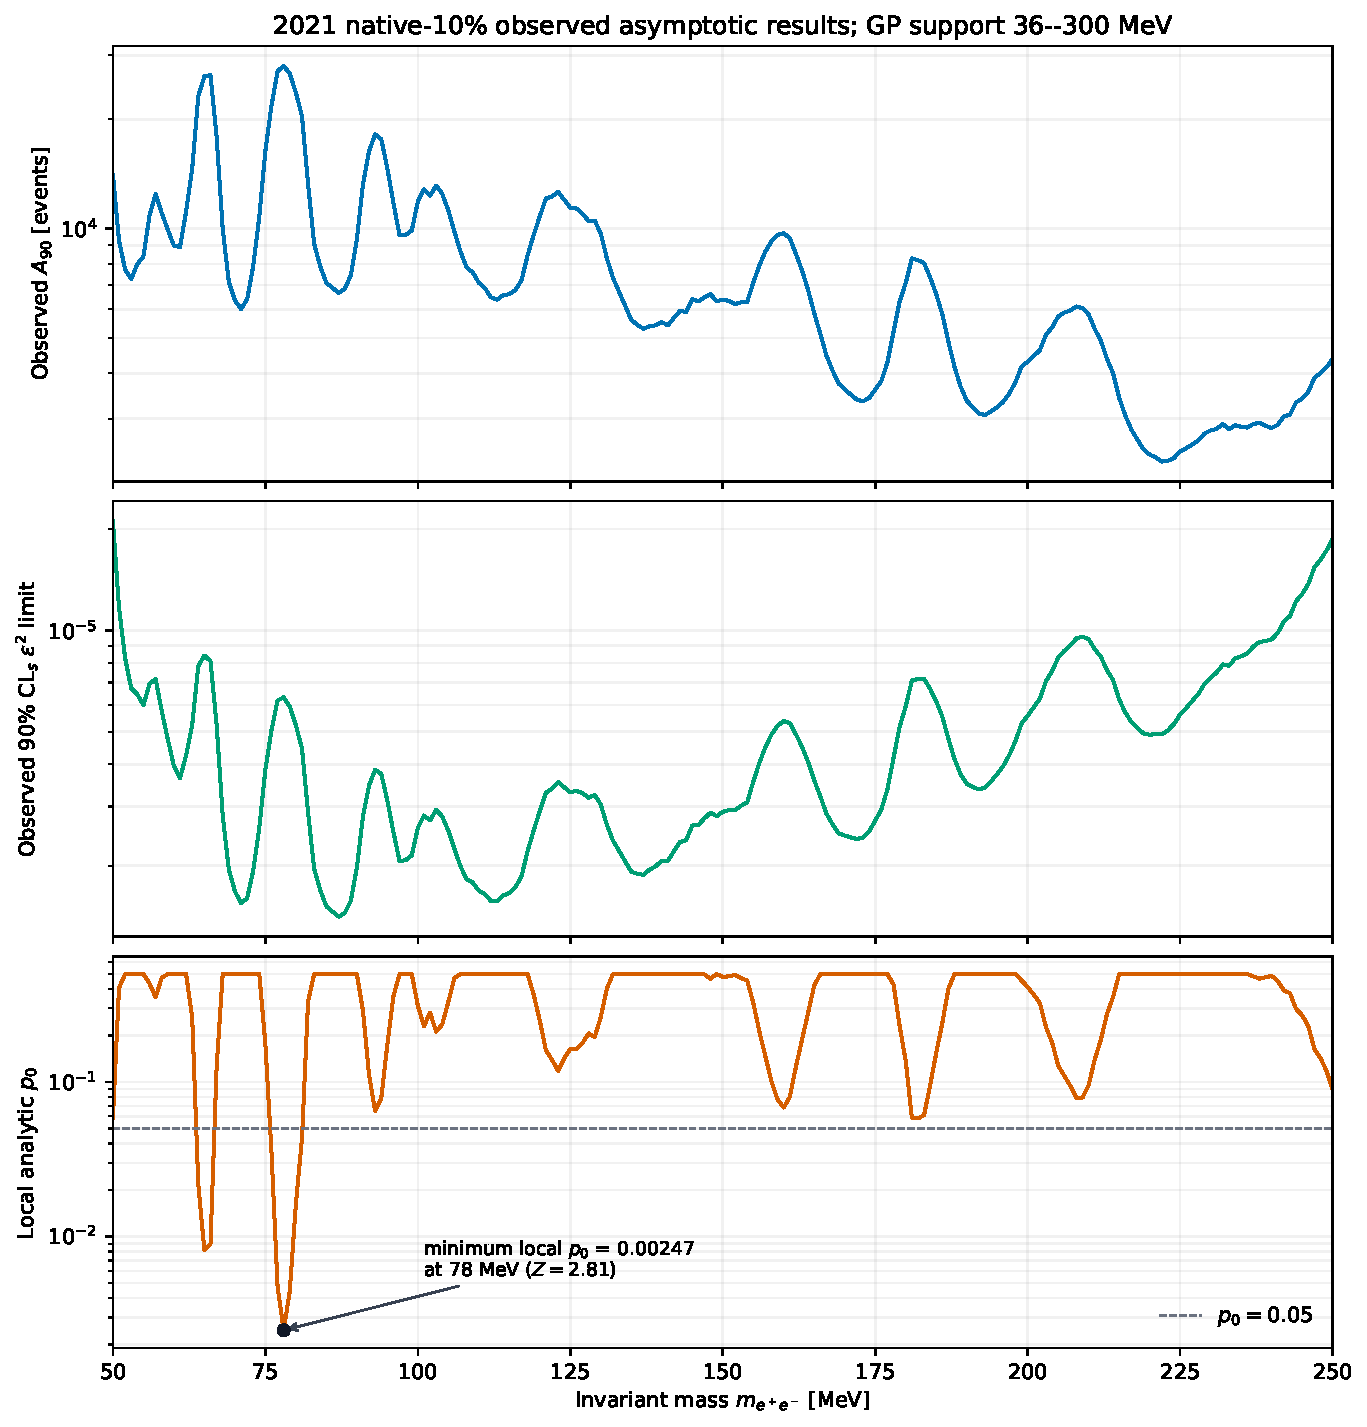
\includegraphics[width=0.98\linewidth]{v4p9p5_support_figs/observed_aligned_yield_eps2_pvalue.pdf}
  \caption{Observed 2021 native-10\% scan with the selected 36--300~MeV GP support.
  The panels show the 90\% \CLs{} signal-yield upper limit, the corresponding
  $\eps^2$ upper limit, and the local analytic $p_0$.  The dashed line in the lower
  panel marks 0.05.  No expected-limit bands are shown, and the minimum local
  $p_0$ is not corrected for the mass scan.}
  \label{fig:v4p9p5-observed}
\end{figure}

The observed yield limits range from 2287 to 28077 events, while the $\eps^2$ limits
range from $1.41\times10^{-6}$ to $2.11\times10^{-5}$.  The smallest local analytic
value is $p_0=0.00247$ at 78~MeV, equivalent to $Z=2.81$ under the local asymptotic
mapping.  This is a local diagnostic, not a global significance: the scan has not been
calibrated with background-only pseudoexperiments or another trials correction.  This
pass also provides no expected-limit bands or direct \CLs{} coverage result.

\FloatBarrier
